\documentclass[12pt]{article}

\usepackage{report}

\usepackage[utf8]{inputenc} % allow utf-8 input
\usepackage[T1]{fontenc}    % use 8-bit T1 fonts
\usepackage[colorlinks=true, linkcolor=black, citecolor=blue, urlcolor=blue]{hyperref}       % hyperlinks
\usepackage{url}            % simple URL typesetting
\usepackage{booktabs}       % professional-quality tables
\usepackage{amsfonts}       % blackboard math symbols
\usepackage{nicefrac}       % compact symbols for 1/2, etc.
\usepackage{microtype}      % microtypography
\usepackage{lipsum}		% Can be removed after putting your text content
\usepackage{graphicx}
\usepackage{natbib}
\usepackage{doi}
\usepackage{listings}
\usepackage{xcolor}
\usepackage{float}
\setcitestyle{aysep={,}}



\title{Project Step 3}

\author{List of Group Members\\
\AND Brandon Markham
\AND Paul Henson
\AND Sam Arshad
\AND
\AND
	CS.3339 Computer Architecture\\
\AND
	Texas State University\\
}

% Uncomment to remove the date
\date{April 16, 2024}

% Uncomment to override  the `A preprint' in the header
\renewcommand{\headeright}{Project Step 3 - Turing Machine}
\renewcommand{\undertitle}{Turing Machine}
\renewcommand{\shorttitle}{Bringing It All Together}

\definecolor{codegreen}{rgb}{0,0.6,0}
\definecolor{codegray}{rgb}{0.5,0.5,0.5}
\definecolor{codepurple}{rgb}{0.58,0,0.82}
\definecolor{backcolour}{rgb}{0.95,0.95,0.92}

\lstdefinestyle{mystyle}{
    backgroundcolor=\color{backcolour},   
    commentstyle=\color{codegreen},
    keywordstyle=\color{magenta},
    numberstyle=\tiny\color{codegray},
    stringstyle=\color{codepurple},
    basicstyle=\ttfamily\footnotesize,
    breakatwhitespace=false,         
    breaklines=true,                 
    captionpos=b,                    
    keepspaces=true,                 
    numbers=left,                    
    numbersep=5pt,                  
    showspaces=false,                
    showstringspaces=false,
    showtabs=false,                  
    tabsize=2
}

\lstset{style=mystyle}


\begin{document}
\maketitle

\newpage
%\tableofcontents
\thispagestyle{empty}


\newpage
\setcounter{page}{1}
\section{Introduction}
For this final step of the project, the Turing Machine group implemented, tested and integrated our Verilog code into one package. We used an online web editor and compiler called "EDA Playground". We implemented behavioral-level logic to accomplish these tasks, and used EDA Playground's waveform generator feature in order to visualize the waveform(s).


\section{Verilog Modules}
\label{sec:headings}
In this section, we were required to assemble each previously-created bitwise logic and arithmetic functions into a top-level ALU module. Each module presented below (outside of the final ALU module) are written and function the same as they did in the previous reports with one exception in the bitshifting operation, which is described in its subsection.\newline\newline

\subsection{MultiBit AND}
\lstinputlisting[language= Verilog]{Verilog/multibit_AND.v}

\subsection{MultiBit NAND}
\lstinputlisting[language= Verilog]{Verilog/multibit_NAND.v}

\subsection{MultiBit OR}
\lstinputlisting[language= Verilog]{Verilog/multibit_OR.v}

\subsection{MultiBit NOR}
\lstinputlisting[language= Verilog]{Verilog/multibit_NOR.v}

\subsection{MultiBit XOR}
\lstinputlisting[language= Verilog]{Verilog/multibit_XOR.v}

\subsection{MultiBit XNOR}
\lstinputlisting[language= Verilog]{Verilog/multibit_XNOR.v}

\subsection{MultiBit NOT}
\lstinputlisting[language= Verilog]{Verilog/multibit_NOT.v}


\subsection{Binary Adder}
\lstinputlisting[language= Verilog]{Verilog/binaryAdder.v}

\subsection{Binary Subtractor}
\lstinputlisting[language= Verilog]{Verilog/binarySubtractor.v}

\subsection{Binary Multiplier}
\lstinputlisting[language= Verilog]{Verilog/binaryMultiplier.v}

\subsection{Binary Dividor}
\lstinputlisting[language= Verilog]{Verilog/binaryDivider.v}

\subsection{Multi Bit Shifter}
Notable Version Change: Lines 22 and 36. The continuation criteria of two for loops were expanded from the previous version in order to create an upper ceiling on the number of loops that were possible to be requested by the control input.
\lstinputlisting[language= Verilog]{Verilog/multiShift.v}

\section{ALU}
The ALU module instantiates each of the modules shown above, and handles routing outputs from the operation selected via an input operation code (opcode).
\lstinputlisting[language= Verilog]{Verilog/ALU.v}


\section{Verilog Testbench}
The testbench was designed in such a way as to be able to test ALU modules with widths of multiples of 4, defined by a WIDTH parameter on line 2 of the testbench file. The tested variables used Verilog's replication operator in order to generate useful input commands of varying length. \\
In testing, the WIDTH parameter was scaled to values 4, 8, 16, and 32 in order to test higher ALU register sizes.
\lstinputlisting[language= Verilog]{Verilog/testBench.v}


%\begin{figure}[h]
%    \centering
%   \includegraphics[width = 1.0\textwidth]{figs/NAND_IMG.jpg}
%    \caption{Nand truth table and gate}
%    \label{fig:enter-label}
%\end{figure}

\newpage

\section{Waveform Test}
Shown below are the output waveform tables generated by testing. \\
Opcode interpretations and "extra" output signal labels have been added to each waveform table image for ease of interpretation.
\subsubsection{GATES}
    \begin{figure}[H]
        \centering
        \includegraphics[width = 1.0\textwidth]{figs/CompArch FInal Test Cases 4x labeled GATES (resized).png}
        \caption{4-bit wide bitwise logic functions.}
        \label{fig:enter-label}
    \end{figure}

\subsubsection{OPERATIONS}
    \begin{figure}[H]
        \centering
        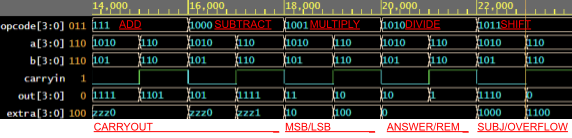
\includegraphics[width = 1.0\textwidth]{figs/CompArch Final Test Cases 4x labeled OPERATIONS (resized).png }
        \caption{4-bit wide arithmetic operations.}
        \label{fig:enter-label}
    \end{figure}

\subsection{Extra Credit: Higher-Width Register Waveforms}

    
\subsubsection{8, 16, 32 bit Gates and Operations}
Higher-width register testing waveforms shown below have signal values listed in hexadecimal to accommodate reasonable viewing.
     \begin{figure}[H]
        \centering
        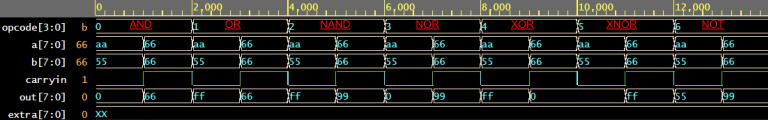
\includegraphics[width = 1.0\textwidth]{figs/CompArch Final Test Cases 8x labeled GATES (resized).png}
        \caption{8-bit wide bitwise logic functions.}
        \label{fig:enter-label}
    \end{figure}
    
   \begin{figure}[H]
        \centering
        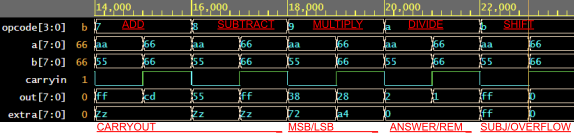
\includegraphics[width = 1.0\textwidth]{figs/CompArch Final Test Cases 8x labeled OPERATIONS (resized).png}
        \caption{8-bit wide arithmetic operations.}
        \label{fig:enter-label}
    \end{figure}


    \begin{figure}[H]
        \centering
        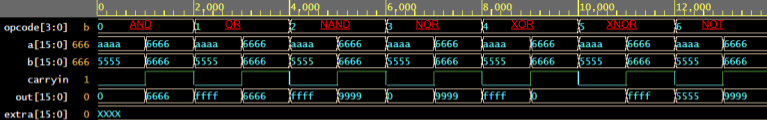
\includegraphics[width = 1.0\textwidth]{figs/CompArch Final Test Cases 16x labeled GATES (resized).png}
        \caption{16-bit wide bitwise logic functions.}
        \label{fig:enter-label}
    \end{figure}

    \begin{figure}[H]
        \centering
        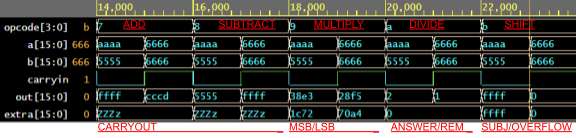
\includegraphics[width = 1.0\textwidth]{figs/CompArch Final Test Cases 16x labeled OPERATIONS (resized).png}
        \caption{16-bit wide arithmetic operations.}
        \label{fig:enter-label}
    \end{figure}


    \begin{figure}[H]
        \centering
        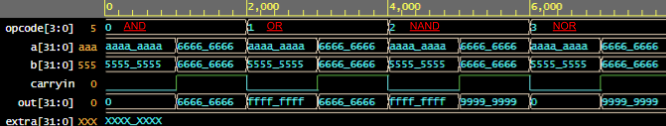
\includegraphics[width = 1.0\textwidth]{figs/CompArch Final Test Cases 32x labeled GATES (resized 1 of 2).png}
        \caption{32-bit wide bitwise logic functions, table 1 of 2.}
        \label{fig:enter-label}
    \end{figure}
    
    \begin{figure}[H]
        \centering
        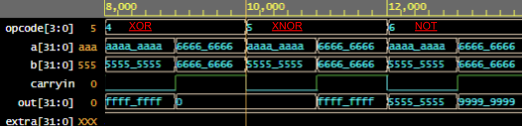
\includegraphics[width = 1.0\textwidth]{figs/CompArch Final Test Cases 32x labeled GATES (resized 2 of 2).png}
        \caption{32-bit wide bitwise logic functions, table 2 of 2.}
        \label{fig:enter-label}
    \end{figure}

    \begin{figure}[H]
        \centering
        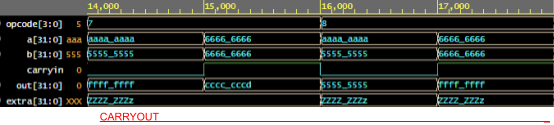
\includegraphics[width = 1.0\textwidth]{figs/CompArch Final Test Cases 32x labeled OPERATIONS (resized 1 of 2).png}
        \caption{32-bit wide arithmetic operations, table 1 of 2. Add and Subtract operations shown in order.}
        \label{fig:enter-label}
    \end{figure}

    \begin{figure}[H]
        \centering
        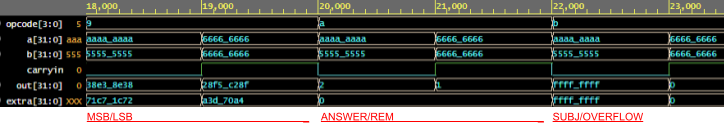
\includegraphics[width = 1.0\textwidth]{figs/CompArch Final Test Cases 32x labeled OPERATIONS (resized 2 of 2).png}
        \caption{32-bit wide arithmetic operations, table 2 of 2. Multiply, Divide, and Bitshift operations shown in order.}
        \label{fig:enter-label}
    \end{figure}



\section{Conclusion}
This final segment of the project required very little extra overhead in terms of learning and work as compared to the previous two parts. The testbench was, by now, a familiar format that required only one novel technique in the form of parametrizable variable generation via the replication operator. \\

Notably, Verilog's switch (case) statement was implemented for the first time in this project inside of the ALU module. Otherwise, only one small adjustment was required between the previously created modules. \\
The majority of the group's effort for this section was in compiling and verifying the outputs of each test case rather than in learning and writing code, which is nonetheless likely representative of many real-world tasks we may encounter in the future. \\ 
\\
As closing notes for the entirety of this project, the members of our group have gained a valuable understanding of both a hardware descriptive language and an advanced markup document-creation language, have gained a sense for the amount of work that must be put in to learn new languages without actively guidance, and have learned a lesson about fully exploring the confines of an assignment and requesting clarification before misguidedly reinventing the wheel.


\end{document}